\documentclass[11pt]{article}
\usepackage{amsmath}
\usepackage{fancyhdr}
\usepackage{hyperref}
\usepackage{graphicx}
\newcommand{\compactlist}{\setlength{\itemsep}{0pt} \setlength{\parskip}{0pt} \setlength{\leftskip}{-1em}}
\usepackage[top=0.9in, bottom=0.8in, left=0.9in, right=0.9in]{geometry}

\lhead{MATH 4263/5373}
\rhead{Sep. 6, 2019}
\chead[RE]{Fixed-point iterations}
\cfoot{}
\rfoot{}%Code for figure and report is (not yet) available in the class folder.}
\pagestyle{fancy}

\begin{document}
%Consider the function \[g(x) = 2^{-x} = e^{-\ln(2)x}\] and the associated fixed-point problem \(g(x) = x\). The result obtained by cobwebbing (graphically) is shown in the figure below, with the iterates marked in ticks on the bottom axis.  Beyond \(n=4\) things get pretty crowded near the fixed point.
%%
%\begin{center}
%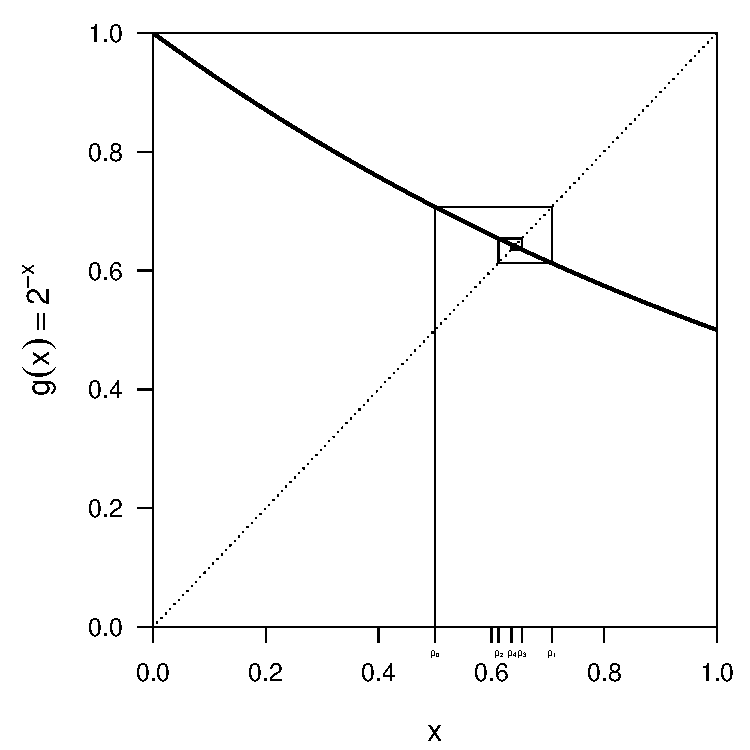
\includegraphics[width=0.75\textwidth]{fixedpoint.pdf}
%\end{center}
%%
%As tabular output we have the first few steps as well. Note that \(p_n\) are approximates the the root \(p\).
%\begin{center}
%\begin{tabular}{cc}
%\(n\) & \(p_n\)\\
%\hline\hline
%0 & 0.5000000\\
%1 & 0.7071068\\
%2 & 0.6125473\\
%3 & 0.6540409\\
%4 & 0.6354978
%\end{tabular}
%\end{center}
%\newpage

Now, for a given degree of accuracy, how many iterations do we actually need?  Consider \[2^{-x}=x\text{ on }\left[\frac{1}{3}, 1\right]\] The bounds are given by \[|p_n-p|\leq k^n \max(p_0-a, b - p_0)\]
using the initial guess, and by \[|p_n-p|\leq\frac{k^n}{1-k}|p_1-p_0|\] using the initial guess and first iteration.  We will look at a few applications of the bounds to the problem above.  First notice that \(g'(x) = -\ln(2)2^{-x}\) and \(|g'(x)| \leq \ln(2)2^{-{1}/{3}} < k = 0.551\), where \(k = 0.551\) is a bound on the magnitude of \(g'(x)\).

The worst possible initial guess would be at one of the endpoints, so we will start there (this maximizes the term \( \max(p_0-a, b - p_0)\), which in this case we actually want to do in order to generate a conservative bound).  Taking \(D\) as the desired accuracy (i.e., an accuracy within \(10^{-D}\)), this gives, 
\begin{align*}
k^n \max(p_0-a, b - p_0) & < 10^{-D}\\
(0.551)^n \left(\frac{2}{3}\right) & < 10^{-D}\\
(0.551)^n  & < \left(\frac{3}{2}\right)10^{-D}\\
n \log(0.551) & < \log\left(\frac{3}{2}\right) - D\\
n  & > \frac{\log\left(\frac{3}{2}\right) - D}{\log(0.551)}
\end{align*}
In the last line, the inequality has been reversed since we are dividing by a negative.  With \(D=4\) this gives \(n > 14.77277\) which requires \(N=15\) steps.

For the second bound, we actually need \(p_1\) in addition to \(p_0\).  From \(p_0 = \frac{2}{3}\), we have \(p_1 = 2^{-1/3}\) (so \(|p_1-p_0| = |2^{-1/3} - \frac{1}{3}| \approx 0.4604\)).  Similarly, from \(p_0=1\), we have \(p_1 = \frac{1}{2}\) (so \(|p_1-p_0| = |\frac{1}{2} - 1| = 0.5\)).  We will use the second of these which is larger in value.
\begin{align*}
\frac{k^n}{1-k}|p_1-p_0| & < 10^{-D}\\
\frac{(0.551)^n}{1-0.551}(0.5) & < 10^{-D}\\
(0.551)^n & < \left(\frac{1-0.551}{0.5}\right) 10^{-D}\\
n\log(0.551) & < \log\left(\frac{1-0.551}{0.5}\right) -D\\
n & > \frac{\log\left(\frac{1-0.551}{0.5}\right) -D}{\log(0.551)}\\
\end{align*}
For consistency, with \(D=4\) this gives \(n > 15.63357\) which requires \(N=16\) steps.  We have to do at least \(16\) steps to ensure we are within the bound, though we may satisfy this much more quickly. Notice that this is quite a bit more work than our bound for the Bisection method required.
\end{document}

%:
%:
%:
%:
%:
%:
